\documentclass[12pt,a4paper]{article}

\input{/home/nick/xelatex.tex}

\usepackage{fontspec}
\usepackage{graphicx}
\usepackage{float}
\usepackage[bottom]{footmisc}
\setmainfont{Minion Pro}

\newcommand{\imagesPath}{/home/nick/arch-ntua/ex03/graphs}


\newcommand{\myWidth}{0.8\linewidth}

\title{Προηγμένα Θέματα Αρχιτεκτονικής Υπολογιστών \\ 3η άσκηση}
\author{Νικόλαος Παγώνας, el18175}
\date{}

\begin{document}
	\maketitle	
	
	\section{Εισαγωγή}
		Στην άσκηση αυτή θα μελετήσουμε τους μηχανισμούς συγχρονισμού και τα πρωτόκολλα συνάφειας κρυφής μνήμης σε σύγχρονες πολυπύρηνες αρχιτεκτονικές, με τη βοήθεια δεδομένου πολυνηματικού κώδικα και του προσομοιωτή \verb|sniper| (ο οποίος αξιοποιεί το \verb|PIN|). 
		
	\section{Εγκατάσταση και χρήση του προσομοιωτή}	
		
		\subsection{Λήψη, εγκατάσταση και παραμετροποίηση του sniper}
			Για την εκτέλεση της άσκησης χρησιμοποιούμε την έκδοση 7.3 του \verb|sniper|, μια έκδοση του \verb|PIN| που περιλαμβάνει και το εργαλείο \verb|pinplay|. Αμφότερες οι εκδόσεις βρίσκονται στο site του εργαστηρίου. Μεταγλωττίζουμε τον sniper σε Ubuntu 22.04, με έκδοση gcc 7. Αφού μεταγλωττίσουμε με επιτυχία τον \verb|sniper|, τον εκτελούμε μέσω του \verb|run-sniper|. Για την παραμετροποίηση χρησιμοποιούμε τα κατάλληλα \verb|.cfg| αρχεία, ή την επιλογή \verb|-g| του \verb|run-sniper|.			
					
		\subsection{McPAT}
			Για τον υπολογισμό της κατανάλωσης ενέργειας χρησιμοποιούμε το \verb|advcomparch_mcpat.py|, μία τροποποιημένη έκδοση του \verb|mcpat.py| που περιέχεται στον \verb|sniper|. Για να το χρησιμοποιήσουμε, το αντιγράφουμε στον φάκελο \verb|sniper-7.3/tools/|. Με αυτό το script μοντελοποιούμε χαρακτηριστικά όπως η κατανάλωση ενέργειας του επεξεργαστή, καθώς και το μέγεθος που καταλαμβάνουν οι δομικές του μονάδες πάνω στο τσιπ.
		
		\subsection{Energy-Delay Product}
			Μία μετρική που θα χρησιμοποιήσουμε στην ανάλυση που ακολουθεί είναι το Energy-Delay Product ($ EDP $). Ορίζεται ως εξής:
			
			\[
				EDP = Energy(J) \cdot runtime(sec)
			\]
			
			και χρησιμοποιείται ώστε να δίνουμε βάρος όχι μόνο στην κατανάλωση ενέργειας, αλλά και στην επίδοση του επεξεργαστή. Παραλλαγές αποτελούν τα $ED^2P, ED^3P$ κ.ο.κ.:
			
			\begin{align*}
				ED^2P &= Energy(J) \cdot runtime^2(sec) \\
				ED^3P &= Energy(J) \cdot runtime^3(sec)
			\end{align*}
	
	\section{Υλοποίηση μηχανισμών συγχρονισμού}
	
		Σε αυτό το σημείο καλούμαστε να υλοποιήσουμε τους μηχανισμούς κλειδώματος \textbf{Test-and-Set (TAS)} και \textbf{Test-and-Test-and-Set (TTAS)}. Στο αρχείο \verb|locks_scalability.c| βρίσκεται κώδικας που χρησιμοποιεί Posix Threads για τη διαχείριση των νημάτων. Κάθε νήμα εκτελεί μία κρίσιμη περιοχή (η είσοδος ελέγχεται από μία κοινή μεταβλητή κλειδιού) για έναν συγκεκριμένο αριθμό επαναλήψεων. Για την απόκτηση και την απελευθέρωση του κλειδιού εκτελούνται οι κατάλληλες ρουτίνες, οι οποίες μπορούν να τροποποιηθούν κατά τη μεταγλώττιση μέσω των flags:
		
		\begin{verbatim}
			-DMUTEX
			-DTAS_CAS
			-DTAS_TS
			-DTTAS_CAS 
			-DTTAS_TS
		\end{verbatim}
		
		\subsection{Υλοποίηση κλειδωμάτων TAS και TTAS}
			Συμπληρώνουμε τις απαιτούμενες υλοποιήσεις στο αρχείο \verb|lock.h|:
			
			\verbatiminput{/home/nick/arch-ntua/ex03/advcomparch-ex3-helpcode/lock.h}
		
		\subsection{Μεταγλώττιση για πραγματικό μηχάνημα ή για προσομοίωση στον sniper}
			Tέλος, σημειώνεται ότι κατά τη μεταγλώττιση μπορούν να δοθούν τα flags:
			
			\begin{verbatim}
				-DSNIPER
				-DREAL
			\end{verbatim}
		
			ανάλογα με το αν επιθυμούμε η εκτέλεση να γίνει σε πραγματικό μηχάνημα, ή να κάνουμε προσομοίωση στον sniper.
	
	\section{Αξιολόγηση επίδοσης}
		
		\subsection{Σύγκριση υλοποιήσεων}
		
			Πολλές φορές οι ρεαλιστικοί περιορισμοί επιβάλλουν κλιμακωσιμότητα χειρότερη της θεωρητικής (που προκύπτει δηλαδή με απλή ανάλυση του αλγορίθμου), ακόμα και για προγράμματα που επιβάλλουν ιδανική κλιμακωσιμότητα\footnote{Με τον όρο "ιδανική κλιμακωσιμότητα" αναφερόμαστε σε προγράμματα που έχουν σχεδιαστεί ώστε ο χρόνος εκτέλεσης με $N$ νήματα να είναι $1/N$ του χρόνου εκτέλεσης για $1$ νήμα.} εκ κατασκευής. Παράγοντες όπως το overhead που προσθέτει το πρωτόκολλο συνάφειας ή το περιορισμένο bandwidth πρόσβασης στην κύρια μνήμη έχουν ως αποτέλεσμα το κόστος μίας λειτουργίας για ένα νήμα (π.χ. πρόσβαση στη μνήμη) να είναι πολύ μεγαλύτερο, όταν συμμετέχουν πολλά νήματα στην εκτέλεση. Για αυτόν τον λόγο ελέγχουμε πειραματικά, τόσο σε προσομοίωση, όσο και στο δικό μας μηχάνημα, την πραγματική κλιμακωσιμότητα του προγράμματος που μεταγλωττίσαμε παραπάνω, ελέγχοντας πλήθος διαφορετικών υλοποιήσεων (διαφορετικοί μηχανισμοί συγχρονισμού, διαφορετικός αριθμός νημάτων, διαφορετικό \verb|grain_size|). Οι συνδυασμοί παραμέτρων και οι αρχιτεκτονικές διαμοιρασμού που χρησιμοποιούνται για τους υπολογισμούς αναγράφονται αναλυτικά στην εκφώνηση της άσκησης.
			
			% 4.1.1			
			\subsubsection{}
			Σε αυτό το μέρος της άσκησης, για κάθε grain size, απεικονίζουμε τον χρόνο εκτέλεσης σε κύκλους συναρτήσει του αριθμού των νημάτων. Σε κάθε διάγραμμα συμπεριλαμβάνονται και οι 5 μηχανισμοί συγχρονισμού (μία καμπύλη για κάθε μηχανισμό). Ακολουθούν τα διαγράμματα \textbf{για grain size ίσο με 1, 10 και 100} αντίστοιχα. Προσοχή στον κατακόρυφο άξονα, τα μεγέθη είναι πολλαπλασιασμένα $\times 10^6, \times 10^8$ κλπ.: 
			
				\begin{figure}[H]
					\begin{center}
						\includegraphics[width=\myWidth]{\imagesPath/4.1.1/grain-1.pdf}
						\caption{Χρόνος εκτέλεσης σε κύκλους συναρτήσει του αριθμού νημάτων, για grain size 1}
					\end{center}
				\end{figure}
			
				\begin{figure}[H]
					\begin{center}
						\includegraphics[width=\myWidth]{\imagesPath/4.1.1/grain-10.pdf}
						\caption{Χρόνος εκτέλεσης σε κύκλους συναρτήσει του αριθμού νημάτων, για grain size 10}
					\end{center}
				\end{figure}
			
				\begin{figure}[H]
					\begin{center}
						\includegraphics[width=\myWidth]{\imagesPath/4.1.1/grain-100.pdf}
						\caption{Χρόνος εκτέλεσης σε κύκλους συναρτήσει του αριθμού νημάτων, για grain size 100}
					\end{center}
				\end{figure}
				
			% 4.1.2
			\subsubsection{}

				Παρατηρούμε ότι οι μηχανισμοί \verb|TAS_CAS| και \verb|TAS_TS| παρουσιάζουν επιδόσεις κοντινές μεταξύ τους, κάτι που είναι λογικό, αφού και οι δύο αποτελούν υλοποιήσεις του μηχανισμού \verb|Test-and-Set|. Όταν δύο ή περισσότεροι επεξεργαστές προσπαθούν να αποκτήσουν το κλείδωμα, οδηγούμαστε σε συνεχόμενες εναλλαγές καταστάσεων (Modified - Invalid) της cache line που περιέχει το κλείδωμα, οπότε δημιουργείται αυξημένη περιττή κίνηση πάνω στο bus. \\
				
				Αντίστοιχα οι μηχανισμοί \verb|TTAS_CAS| και \verb|TTAS_TS| υλοποιούν τον μηχανισμό \verb|Test-and-Test-and-Set|, οπότε και πάλι οι επιδόσεις τους είναι πολύ παραπλήσιες. Η διαφορά με τον μηχανισμό \verb|Test-and-Set| είναι ότι δεν γράφουν συνεχώς πάνω στο κλείδωμα. Αντίθετα, εκτελούν πρώτα ένα load για να δουν αν είναι ελεύθερο το κλείδωμα (test), και μόνο όταν είναι ελεύθερο δοκιμάζουν να το γράψουν/δεσμεύσουν ατομικά (test-and-set). Έτσι, όταν το κλείδωμα δεν είναι διαθέσιμο οι επεξεργαστές κάνουν spin τοπικά (στην cache τους), οπότε αποφεύγεται η ανούσια ευρυεκπομπή στον διάδρομο. Γι' αυτό τον λόγο είναι αναμενόμενο να οι μηχανισμοί \verb|TTAS| να έχουν καλύτερη κλιμακωσιμότητα από τους άλλους. \\
				
				Από τα παραπάνω διαγράμματα φαίνεται ότι οι χρόνος εκτέλεσης είναι (σχεδόν) γραμμική συνάρτηση του πλήθους των νημάτων (μικρή απόκλιση από την γραμμικότητα παρατηρείται για grain size ίσο με 1). Βέβαια, οι κλίσεις των ευθειών αλλάζουν ανάλογα τον μηχανισμό συγχρονισμού. \\
				
				Τη χειρότερη κλιμακωσιμότητα έχει ο μηχανισμός \verb|MUTEX|, για όλα τα grain sizes (αν και οι μηχανισμοί \verb|TAS_CAS & TAS_TS| πλησιάζουν το \verb|MUTEX| για grain size ίσο με 10). Όπως είναι λογικό, ακολουθούν οι μηχανισμοί \verb|TAS_CAS & TAS_TS| (καλύτεροι από \verb|MUTEX| αλλά χειρότεροι από \verb|TTAS_CAS & TTAS_TS|), ενώ οι καλύτεροι είναι οι μηχανισμοί \verb|TTAS_CAS & TTAS_TS|. \\
				
				Επιπλέον παρατηρούμε ότι η αύξηση του grain size (πλήθος dummy υπολογισμών) προκαλεί βελτίωση τόσο της γραμμικότητας, όσο και της κλίσης των ευθειών (ιδιαίτερα το \verb|MUTEX| βελτιώνεται πολύ, αν συγκρίνουμε την μεγάλη του απόκλιση από την γραμμικότητα για grain size ίσο με 1). Αυτό συμβαίνει επειδή αφιερώνεται περισσότερος χρόνος σε "ωφέλιμους" υπολογισμούς, και λιγότερος χρόνος σε ανταγωνισμό των threads για απόκτηση του κλειδώματος, οπότε η επίδοση βελτιώνεται. \\
				
				Φυσικά, περισσότεροι dummy υπολογισμοί σημαίνουν μεγαλύτερος χρόνος εκτέλεσης (αύξηση $\approx$1 τάξη μεγέθους ανά δεκαπλασιασμό του grain size).
			
			% 4.1.3
			\subsubsection{}
				Εδώ, χρησιμοποιούμε το \verb|McPAT| για να απεικονίσουμε την κατανάλωση ενέργειας και το EDP, \textbf{για grain size ίσο με 1, 10 και 100} αντίστοιχα. \\
				
				\begin{figure}[H]
					\begin{center}
						\includegraphics[width=\myWidth]{\imagesPath/4.1.3/grain-1.pdf}
						\caption{Κατανάλωση ενέργειας και EDP, για grain size ίσο με 1}
					\end{center}
				\end{figure}
			
				\begin{figure}[H]
					\begin{center}
						\includegraphics[width=\myWidth]{\imagesPath/4.1.3/grain-10.pdf}
						\caption{Κατανάλωση ενέργειας και EDP, για grain size ίσο με 10}
					\end{center}
				\end{figure}
							
				\begin{figure}[H]
					\begin{center}
						\includegraphics[width=\myWidth]{\imagesPath/4.1.3/grain-100.pdf}
						\caption{Κατανάλωση ενέργειας και EDP, για grain size ίσο με 100}
					\end{center}
				\end{figure}
			
			\subsubsection*{Παρατηρήσεις - Συμπεράσματα}				
				Παρατηρούμε μία αύξηση της ενέργειας που θα μπορούσε να χαρακτηριστεί εκθετική. Ειδικά η αύξηση της ενέργειας από 8 σε 16 νήματα είναι αξιοσημείωτη. Επιπλέον, για grain size 10 και 100, οι μηχανισμοί \verb|TTAS_CAS & TTAS_TS| καταναλώνουν αρκετά περισσότερη ενέργεια σε σχέση με τους υπόλοιπους μηχανισμούς, για μεγάλο αριθμό νημάτων (8-16). Αυτό είναι λογικό, αφού οι μηχανισμοί αυτοί εκτελούν συνεχόμενα reads, τα οποία έχουν μεγαλύτερο ενεργειακό κόστος σε σχέση με τα stalls που προκαλεί ένα cache miss/κατειλημμένο bus στις \verb|Test-and-Set| υλοποιήσεις. Γενικά, φθηνότερος από άποψη ενεργειακής κατανάλωσης φαίνεται πως είναι ο μηχανισμός \verb|TAS|. \\
				
				Όσον αφορά το EDP, οι μηχανισμοί έχουν παραπλήσεις επιδόσεις για grain size 10, ωστόσο καλύτερο EDP γενικά επιτυγχάνουν οι μηχανισμοί \verb|TAS|. Τέλος, ο μηχανισμός \verb|MUTEX| έχει σταθερά το χειρότερο EDP, για μεγάλο πλήθος νημάτων (8-16).
				
			% 4.1.4
			\subsubsection{}
				Σε αυτό το σημείο μεταγλωττίζουμε τις διαφορετικές εκδόσεις του κώδικα για \textbf{πραγματικό} σύστημα. Να σημειωθεί εδώ ότι \textbf{το πραγματικό μηχάνημα μας επιτρέπει να χρησιμοποιήσουμε μέχρι 8 νήματα} (αντί για 16 που είχαμε στα προηγούμενα πειράματα). Χρησιμοποιούμε τις ίδιες παραμέτρους με πριν, με τη διαφορά ότι ο αριθμός επαναλήψεων είναι κατά πολύ αυξημένος (150.000.000), ώστε να μπορούμε να μετρήσουμε με ακρίβεια τον χρόνο εκτέλεσης.
			
				\begin{figure}[H]
					\begin{center}
						\includegraphics[width=\myWidth]{\imagesPath/4.1.4/grain-1.pdf}
						\caption{Χρόνος εκτέλεσης σε δευτερόλεπτα (πραγματικό σύστημα), για grain size ίσο με 1}
					\end{center}
				\end{figure}
			
				\begin{figure}[H]
					\begin{center}
						\includegraphics[width=\myWidth]{\imagesPath/4.1.4/grain-10.pdf}
						\caption{Χρόνος εκτέλεσης σε δευτερόλεπτα (πραγματικό σύστημα), για grain size ίσο με 10}
					\end{center}
				\end{figure}
			
				\begin{figure}[H]
					\begin{center}
						\includegraphics[width=\myWidth]{\imagesPath/4.1.4/grain-100.pdf}
						\caption{Χρόνος εκτέλεσης σε δευτερόλεπτα (πραγματικό σύστημα), για grain size ίσο με 100}
					\end{center}
				\end{figure}
			
			\subsubsection*{Παρατηρήσεις - Συμπεράσματα}
				Κι εδώ παρατηρούμε γραμμική κλιμάκωση, όπως και στην περίπτωση που είχαμε προσομοίωση με τον sniper. Σημαντική απόκλιση από την γραμμικότητα έχουμε μόνο κατά τη μετάβαση από 4 σε 8 νήματα για grain size ίσο με 1, και για τους μηχανισμούς \verb|TAS_CAS & TAS_TS|. Αυτή τη φορά βέβαια, οι μηχανισμοί \verb|TTAS| έχουν σημαντικά καλύτερη επίδοση. Ειδικά για grain size ίσο με 1, ο χρόνος παραμένει σχεδόν σταθερός με αύξηση των νημάτων. \\
				
				Άξιο προσοχής είναι επίσης το γεγονός ότι οι δύο μηχανισμοί \verb|TAS_CAS & TAS_TS| αποκλίνουν σημαντικά στην επίδοση τους, όσο αυξάνεται ο αριθμός των νημάτων. Αυτή η διαφορά φαίνεται να εκφυλίζεται όσο αυξάνεται το grain size. Μάλιστα, η επίδοση των \verb|TAS| μηχανισμών είναι χειρότερη από αυτή του \verb|MUTEX|. Τέλος, σημαντικό είναι επίσης το ότι ο μηχανισμός \verb|MUTEX| έχει παραπλήσια επίδοση με τους \verb|TTAS| μηχανισμούς, για grain size ίσο με 1. \\
				
		\subsection{Τοπολογία νημάτων}
			
			% 4.2.1
			\subsubsection{}
				Στο ερώτημα αυτό σκοπός είναι να αξιολογήσουμε την κλιμάκωση των διαφόρων υλοποιήσεων όταν τα νήματα εκτελούνται σε πυρήνες με διαφορετικά χαρακτηριστικά ως προς τον διαμοιρασμό των πόρων. Επιλέγουμε 1000 iterations, 4 threads, και grain size ίσο με 1. Εξετάζουμε τις τοπολογίες:
				
				\begin{itemize}
					\item \textbf{share-all}: και τα 4 νήματα βρίσκονται σε πυρήνες με κοινή L2 cache
					\item \textbf{share-L3}: και τα 4 νήματα βρίσκονται σε πυρήνες με κοινή L3 cache, αλλά όχι κοινή L2 cache
					\item \textbf{share-nothing}: και τα 4 νήματα βρίσκονται σε πυρήνες με διαφορετική L3 cache
				\end{itemize}
				
				Ακολουθούν κατά σειρά τα διαγράμματα:
				
				\begin{itemize}
					\item Κύκλοι ρολογιού 
					\item Κατανάλωση ενέργειας
					\item EDP
				\end{itemize}
			
				Για κάθε μηχανισμό συγχρονισμού, απεικονίζονται οι 3 τοπολογίες share-all/L3/nothing. Προσοχή στον κατακόρυφο άξονα, τα μεγέθη είναι πολλαπλασιασμένα $\times 10^6, \times 10^{-6}$ κλπ: 
				
				\begin{figure}[H]
					\begin{center}
						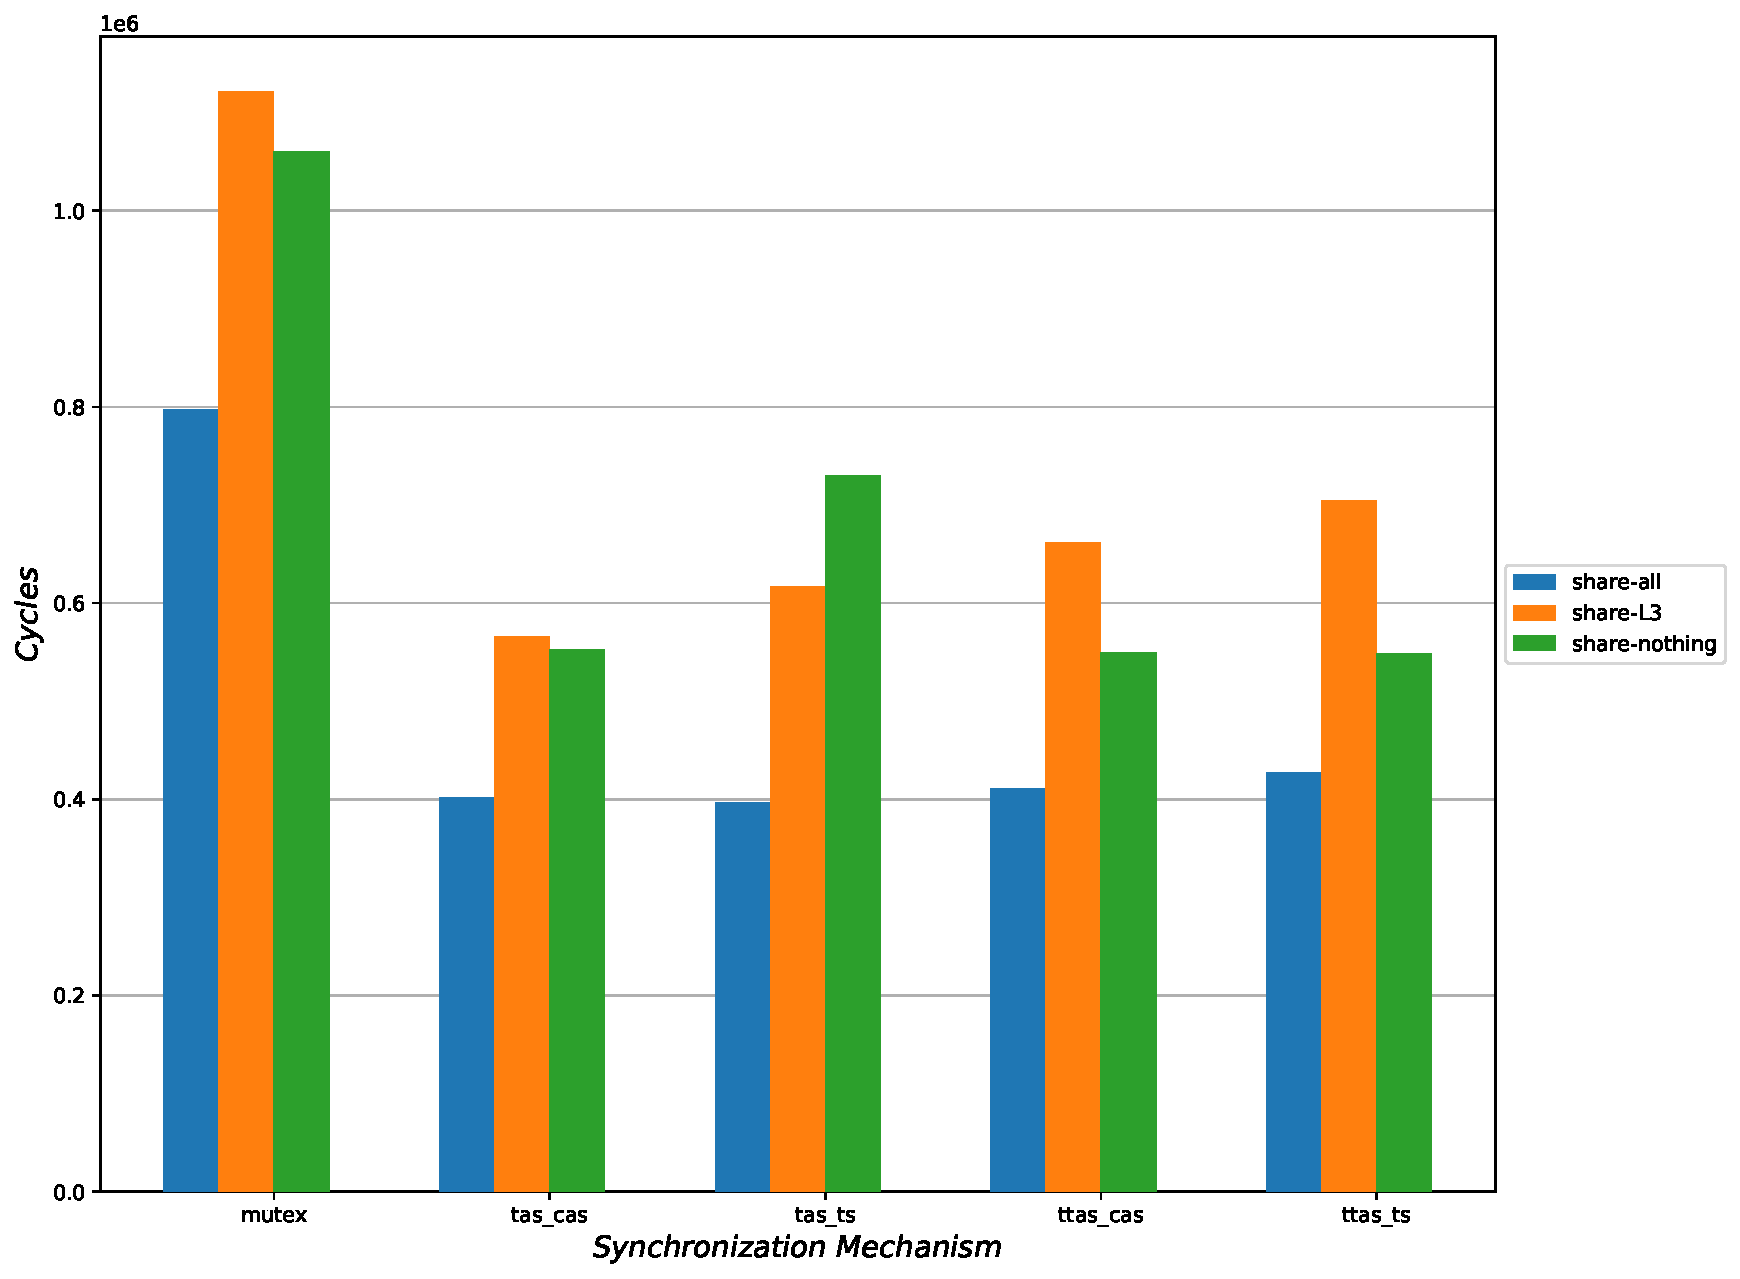
\includegraphics[width=\myWidth]{\imagesPath/4.2.1/topology-time-analysis.pdf}
						\caption{Χρόνος εκτέλεσης σε κύκλους}	
				\end{center}
				\end{figure}
			
				\begin{figure}[H]
					\begin{center}
						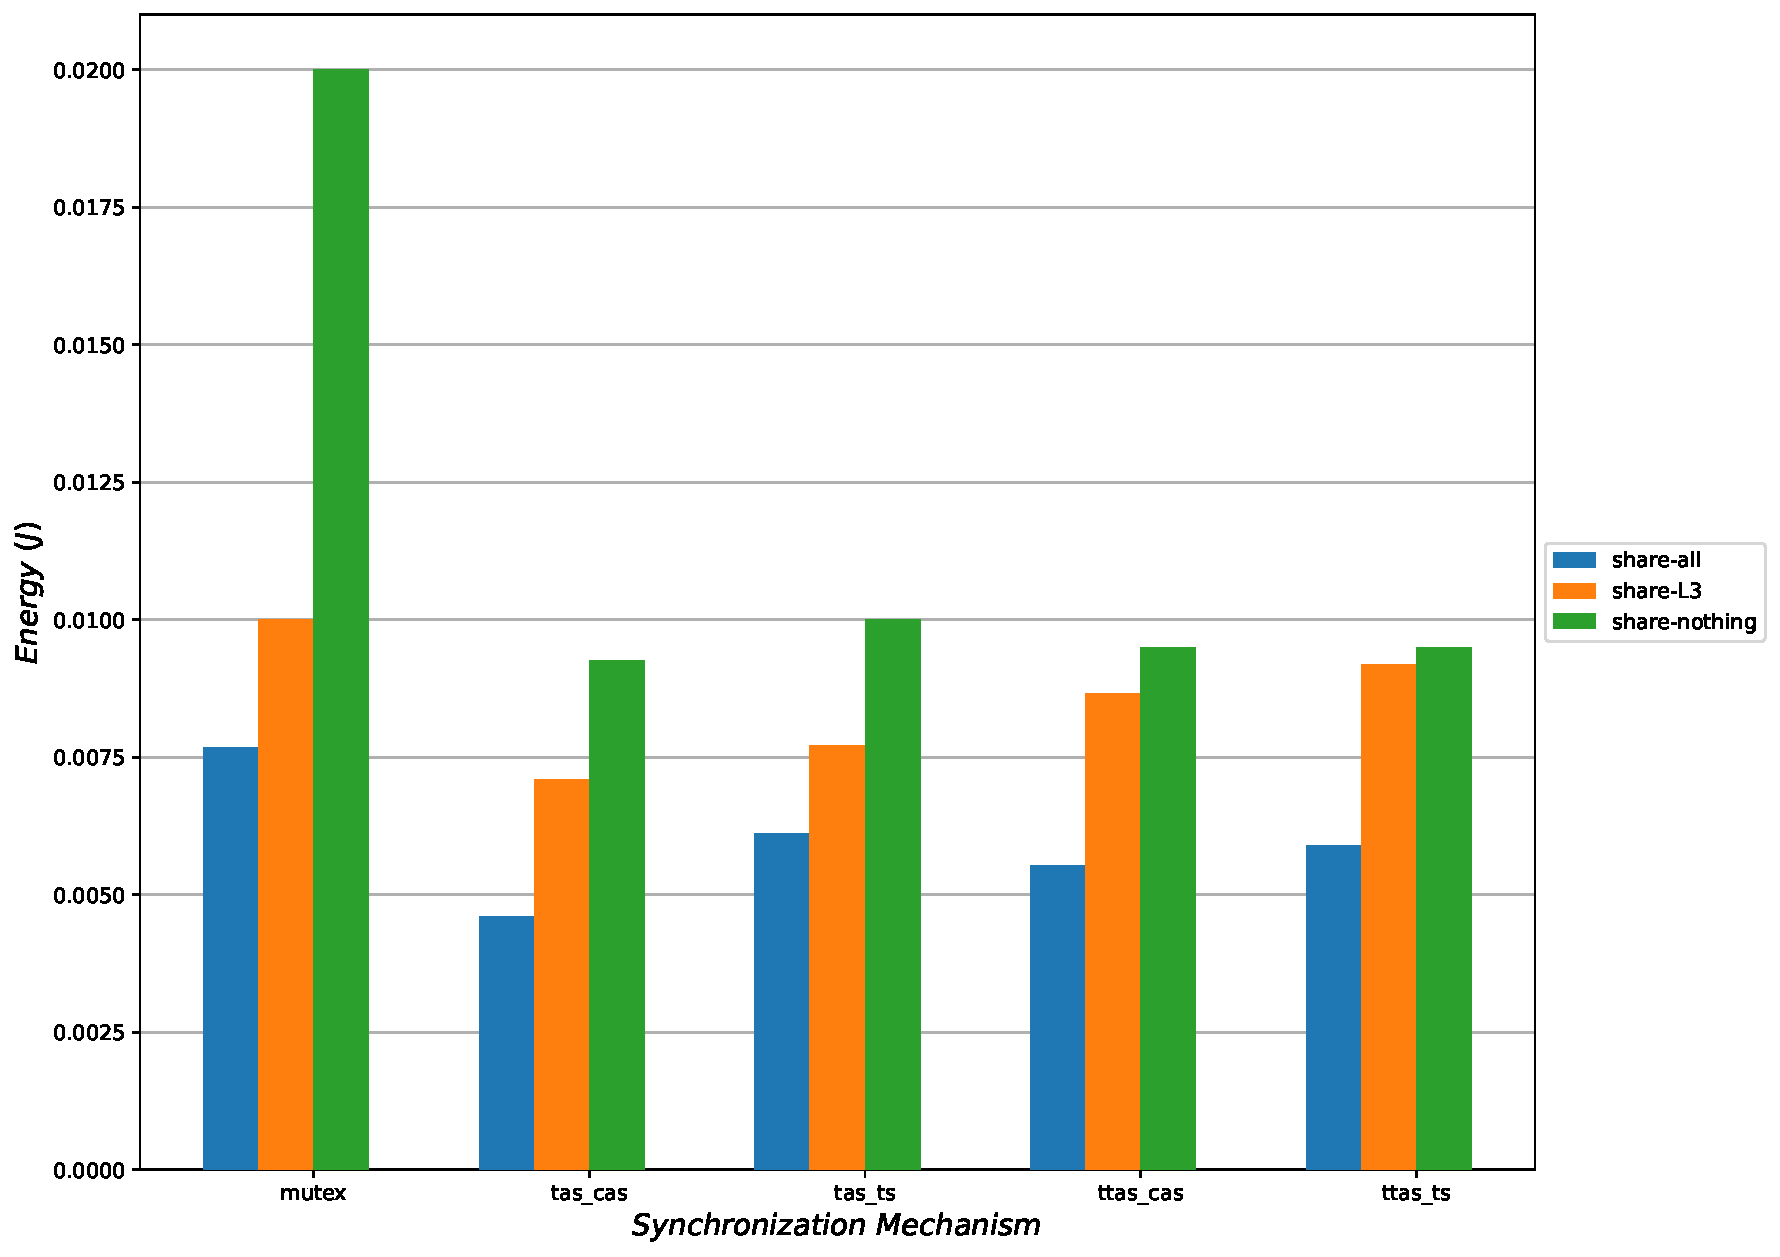
\includegraphics[width=\myWidth]{\imagesPath/4.2.1/topology-energy-analysis.pdf}
						\caption{Κατανάλωση ενέργειας σε J}
					\end{center}
				\end{figure}
			
				\begin{figure}[H]
					\begin{center}
						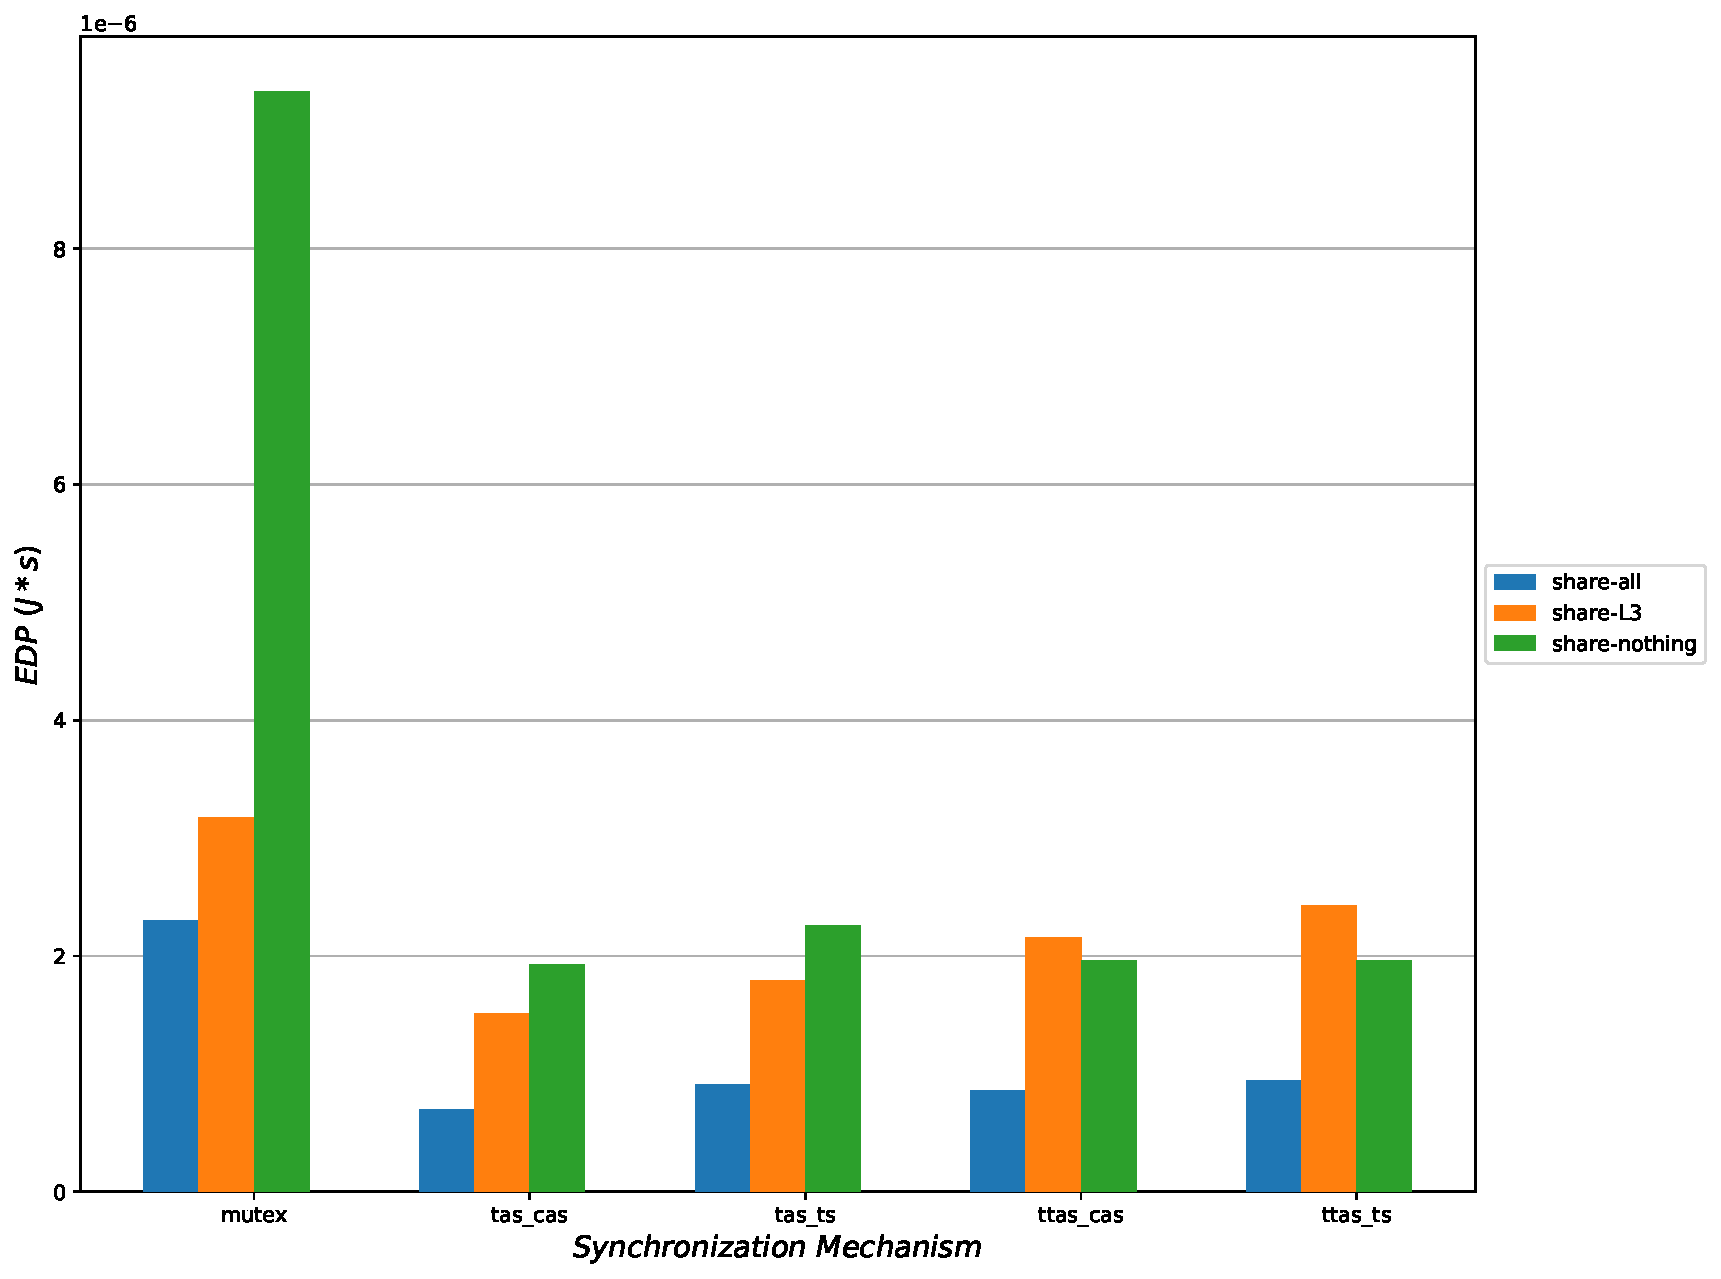
\includegraphics[width=\myWidth]{\imagesPath/4.2.1/topology-edp-analysis.pdf}
						\caption{EDP σε J $\times$ sec}	
					\end{center}
				\end{figure}
			
			\subsubsection*{Παρατηρήσεις - Συμπεράσματα}

				Όσον αφορά τον χρόνο εκτέλεσης, για όλους τους μηχανισμούς συγχρονισμού η καλύτερη επίδοση επιτυγχάνεται με την τοπολογία share-all. Για τους μηχανισμούς \verb|MUTEX, TAS_TS, TAS_CAS| ακολουθεί η τοπολογία share-L3 και ύστερα η share-nothing. Αντίθετα, για τους μηχανισμούς \verb|TTAS_TS & TTAS_CAS| ακολουθεί η τοπολογία share-nothing, και ύστερα η share-L3. \\
				
				Ο λόγος για τον οποίο η share-all τοπολογία είναι βέλτιστη είναι επειδή αν ο επεξεργαστής ζητήσει ένα invalid cache line, τότε θα ενημερωθεί η ιεραρχία μέχρι την L2, και ύστερα θα διαβαστεί από εκεί το δεδομένο, ενώ στο share-L3 η invalid cache line θα ζητηθεί από την L3, και αντίστοιχα στο share-nothing θα χρειαστεί να φτάσουμε μέχρι την κύρια μνήμη, οπότε ο χρόνος που απαιτείται αυξάνεται σημαντικά. \\
				
				Όσον αφορά την μετρική της ενέργειας, η τοπολογία share-all έχει την μικρότερη κατανάλωση, ενώ η share-nothing έχει την μεγαλύτερη κατανάλωση. Αντίστοιχα για το EDP, καλύτερη επίδοση έχει η τοπολογία share-all (ελάχιστο προβάδισμα έχει η τοπολογία share-L3 στις περιπτώσεις \verb|TTAS_CAS & TTAS_TS|), ενώ την χειρότερη η τοπολογία share-nothing. 
\end{document}